\section{Implementação}

A implementação dos métodos de busca de raízes foi desenvolvida em Python,
utilizando bibliotecas como \texttt{ttkbootstrap} para a interface gráfica e
\texttt{matplotlib} para a visualização dos métodos em ação. O código está
estruturado em três arquivos principais: \texttt{app.py}, \texttt{ui.py} e
\texttt{functions.py}.

\subsection{Visão Geral}

A estrutura do código é organizada da seguinte forma:
\begin{itemize}
	\item \textbf{app.py}: Ponto de entrada da aplicação, responsável por inicializar a interface gráfica.
	\item \textbf{ui.py}: Contém a implementação da interface gráfica e gerencia a interação do usuário.
	\item \textbf{functions.py}: Implementa os métodos numéricos de busca de raízes e fornece suporte para os cálculos.
\end{itemize}

\subsection{Interface}

A interface gráfica do aplicativo foi implementada no arquivo \texttt{ui.py},
utilizando a biblioteca \texttt{ttkbootstrap} para um design moderno e
intuitivo. A interface permite ao usuário inserir uma função \( f(x) \), definir
um intervalo ou chute inicial, escolher um método de busca de raízes e
visualizar os resultados tanto numericamente quanto graficamente.

O código é estruturado em três classes principais:
\begin{itemize}
	\item \textbf{RootFinderUI}: Gerencia a interface principal, incluindo
	      campos de entrada, botões de ação e a exibição dos resultados.
	\item \textbf{PlotManager}: Responsável por gerar e atualizar os gráficos
	      das funções e dos métodos utilizados.
	\item \textbf{ThemeManager}: Permite alternar entre temas claros e escuros
	      para melhor experiência visual.
\end{itemize}

\subsubsection{RootFinderUI: Estrutura da Interface}

A classe \texttt{RootFinderUI} define os elementos principais da interface e
gerencia as interações do usuário. A inicialização ocorre no método
\texttt{\_\_init\_\_}, onde são criados os seguintes componentes:
\begin{itemize}
	\item Campos de entrada para a função \( f(x) \), \( g(x) \) (caso
	      necessário), intervalo \([a, b]\) ou chute inicial e tolerância.
	\item Um menu suspenso para selecionar o método numérico desejado.
	\item Botões para executar a busca da raiz, copiar os resultados, salvar o
	      gráfico e alternar o tema.
	\item Um rótulo para exibir os resultados numéricos.
	\item Uma área gráfica onde a função e a raiz encontrada são plotadas.
\end{itemize}

O trecho de código abaixo demonstra a criação do campo de entrada para a função
\( f(x) \):

\hrule
\lstset{style=mystyle}
\begin{lstlisting}[language=Python]
ttk.Label(input_frame, text="f(x):").grid(row=0, column=0, sticky="w")
self.f_entry = ttk.Entry(input_frame, width=40)
self.f_entry.grid(row=0, column=1, columnspan=3)
self.f_entry.insert(0, "sin(x) + cos(x) + 1")
\end{lstlisting}
\hrule

A entrada padrão para a função é \( f(x) = \sin(x) + \cos(x) + 1 \), podendo ser
alterada pelo usuário.

\subsubsection{Seleção de Método e Ajuste de Parâmetros}

Os métodos disponíveis são carregados automaticamente a partir da classe
\texttt{RootFinderMethods}, permitindo que novos algoritmos sejam adicionados
sem necessidade de modificar a interface:

\hrule
\lstset{style=mystyle}
\begin{lstlisting}[language=Python]
self.methods = self._get_root_finding_methods()
self.method_combobox = ttk.Combobox(
    input_frame, textvariable=self.method_var, values=list(self.methods.keys())
)
\end{lstlisting}
\hrule

A função \texttt{\_get\_root\_finding\_methods} percorre os métodos definidos na
classe \texttt{RootFinderMethods} e os adiciona à interface permitindo
selecionar funções a ignorar.

\subsubsection{Execução do Cálculo e Exibição dos Resultados}

Ao pressionar o botão "Solve", o método \texttt{solve} é chamado, realizando as
seguintes operações:
\begin{enumerate}
	\item Obtém os valores inseridos pelo usuário.
	\item Converte a função de string para código executável usando
	      \texttt{eval}.
	\item Chama o método apropriado de \texttt{RootFinderMethods}.
	\item Exibe a raiz encontrada e o número de iterações.
	\item Atualiza o gráfico com a função e a raiz.
\end{enumerate}

O código abaixo ilustra como a solução é processada:

\hrule
\lstset{style=mystyle}
\begin{lstlisting}[language=Python]
root, iterations, computation_time = self.function_solver.solve(
    f_str, a, b, tol, method_name, g_str
)
result_text = f"Root: {root:.6f}\nIterations: {iterations}\nTime: {computation_time:.6f} s"
self.result_label.config(text=result_text)
\end{lstlisting}
\hrule

Se um erro for encontrado (como ausência de mudanças de sinal no método da
bisseção), uma mensagem de erro é exibida ao usuário.

\subsubsection{Gerenciamento da Visualização Gráfica}

A classe \texttt{PlotManager} é responsável por criar e atualizar os gráficos. O
método \texttt{update\_plot} traça a função no intervalo fornecido e destaca a
raiz encontrada:

\hrule
\lstset{style=mystyle}
\begin{lstlisting}[language=Python]
x = np.linspace(a, b, 400)
y = [self._eval_function(f_str, xi) for xi in x]
self.ax.plot(x, y, label=f"f(x) = {f_str}")
self.ax.scatter([root], [0], color="red", label="Root")
self.ax.axhline(0, color="black", linewidth=0.5)
\end{lstlisting}
\hrule

Além disso, um botão permite salvar o gráfico gerado para análise posterior.

\subsubsection{Personalização da Aparência}

Para melhorar a usabilidade, a classe \texttt{ThemeManager} gerencia os esquemas
de cores do aplicativo. Dois temas estão disponíveis: um claro e um escuro,
alternáveis pelo usuário.

O código abaixo ilustra a alternância de temas:

\hrule
\lstset{style=mystyle}
\begin{lstlisting}[language=Python]
def toggle_theme(self):
    self.current_theme = "minty" if self.current_theme == "darkly" else "darkly"
    self.style.theme_use(self.current_theme)
\end{lstlisting}
\hrule

\subsubsection{Resumo}

A interface do aplicativo proporciona uma experiência interativa e intuitiva
para explorar diferentes métodos numéricos de busca de raízes. Os usuários podem
visualizar o comportamento das funções e comparar a eficiência dos algoritmos de
forma dinâmica.

\subsection{Funções}

Os métodos numéricos utilizados para encontrar raízes de funções foram
implementados no arquivo \texttt{functions.py}. A implementação está organizada
na classe \texttt{RootFinderMethods}, que contém cada método como uma função
estática, permitindo chamadas diretas sem necessidade de instanciar objetos.

Além disso, o módulo inclui a classe \texttt{FunctionSolver}, responsável por
interpretar a função fornecida pelo usuário, selecionar o método adequado e
gerenciar a execução dos cálculos. Essa organização modular facilita a
reutilização e a extensão do código, permitindo adicionar novos métodos sem
impactar a estrutura principal.

A seguir, são detalhadas as implementações de cada método, explicando suas
operações e como os parâmetros de entrada são utilizados para conduzir o
processo iterativo de busca da raiz.

\subsubsection{Bisseção}

A função \texttt{bisection} recebe como entrada uma função \( f \), um intervalo
inicial \([a, b]\), uma tolerância e um número máximo de iterações. O código
inicia verificando se \( f(a) \) e \( f(b) \) possuem sinais opostos. Caso
contrário, uma exceção é levantada.

O loop principal divide o intervalo ao meio repetidamente até que a raiz seja
encontrada dentro da tolerância ou o número máximo de iterações seja atingido. A
cada iteração:

\begin{enumerate}
	\item O ponto médio \( c \) do intervalo é calculado.
	\item Se \( f(c) \) for zero, a raiz foi encontrada.
	\item Caso contrário, o intervalo é reduzido dependendo do sinal de \( f(c) \).
\end{enumerate}

\hrule
\lstset{style=mystyle}
\begin{lstlisting}[language=Python]
@staticmethod
def bisection(f, a, b, tol=1e-6, max_iter=100):
    if f(a) * f(b) >= 0:
        raise ValueError("The function must have opposite signs at the endpoints.")
    iterations = 0
    while (b - a) / 2 > tol and iterations < max_iter:
        c = (a + b) / 2
        if f(c) == 0:
            break
        elif f(c) * f(a) < 0:
            b = c
        else:
            a = c
        iterations += 1
    return (a + b) / 2, iterations
\end{lstlisting}
\hrule

\subsubsection{Newton-Raphson}

A função \texttt{newton\_raphson} recebe uma função \( f \), um chute inicial \(
x_0 \), uma tolerância e um número máximo de iterações. A cada iteração:

\begin{enumerate}
	\item Calcula-se a derivada numérica de \( f \) no ponto atual \( x_0 \).
	\item Se a derivada for muito pequena, o algoritmo para para evitar divisões por valores próximos de zero.
	\item O próximo valor de \( x_0 \) é calculado usando a equação \( x_1 = x_0 - f(x_0) / f'(x_0) \).
\end{enumerate}

O processo continua até que o valor de \( f(x) \) esteja dentro da tolerância ou
que o número máximo de iterações seja atingido.

\hrule
\lstset{style=mystyle}
\begin{lstlisting}[language=Python]
@staticmethod
def newton_raphson(f, x0, tol=1e-6, max_iter=100):
    iterations = 0
    while abs(f(x0)) > tol and iterations < max_iter:
        df = RootFinderMethods.numerical_derivative(f, x0)
        if abs(df) < 1e-10:
            raise ValueError(
                "Derivative is too close to zero. Choose a better interval or initial guess."
            )
        x0 = x0 - f(x0) / df
        iterations += 1
    return x0, iterations
\end{lstlisting}
\hrule

\subsubsection{Falsa Posição}

A função \texttt{false\_position} segue a mesma estrutura da bisseção, mas em
vez de dividir o intervalo ao meio, calcula um novo ponto \( c \) através de
interpolação linear:
\[
	c = b - \frac{f(b) \cdot (b - a)}{f(b) - f(a)}
\]
Esse novo valor é usado para reduzir o intervalo da mesma forma que na bisseção.

\hrule
\lstset{style=mystyle}
\begin{lstlisting}[language=Python]
@staticmethod
def false_position(f, a, b, tol=1e-6, max_iter=100):
    if f(a) * f(b) >= 0:
        raise ValueError("The function must have opposite signs at the endpoints.")
    iterations = 0
    c = a
    while abs(b - a) > tol and iterations < max_iter:
        c = b - f(b) * (b - a) / (f(b) - f(a))
        if abs(f(c)) < tol:
            break
        if f(c) * f(a) < 0:
            b = c
        else:
            a = c
        iterations += 1
    return c, iterations
\end{lstlisting}
\hrule

\subsubsection{Ponto Fixo}

A função \texttt{fixed\_point} recebe como entrada a função iterativa \( g(x)
\), um chute inicial \( x_0 \), uma tolerância e um número máximo de iterações.
A cada iteração, a função \( g(x) \) é aplicada para gerar um novo valor até que
a diferença entre duas iterações consecutivas seja menor do que a tolerância
especificada.

\hrule
\lstset{style=mystyle}
\begin{lstlisting}[language=Python]
@staticmethod
def fixed_point(_, g, x0, tol=1e-6, max_iter=100):
    iterations = 0
    x1 = x0
    while iterations < max_iter:
        x1 = g(x0)  # Aplica a função iterativa g(x)
        if abs(x1 - x0) < tol:
            return x1, iterations
        x0 = x1
        iterations += 1
    raise ValueError("Fixed-point iteration did not converge.")
\end{lstlisting}
\hrule

O código segue os seguintes passos:
\begin{itemize}
	\item A variável \texttt{iterations} inicia em zero e serve como contador de
	      iterações.
	\item O loop \texttt{while} continua até que o número máximo de iterações
	      seja atingido.
	\item A cada iteração, \texttt{x1} recebe o valor gerado por \texttt{g(x0)},
	      atualizando a estimativa da raiz.
	\item O critério de parada verifica se \( |x_1 - x_0| \) é menor do que a
	      tolerância \texttt{tol}, indicando convergência.
	\item Caso o critério de parada seja atendido, a função retorna o valor de
	      \texttt{x1} e o número de iterações realizadas.
	\item Se o método não convergir dentro do limite de iterações, a função
	      lança um erro informando que a iteração falhou.
\end{itemize}

\subsubsection{Secante}

A função \texttt{secant} aproxima a derivada de \( f(x) \) através da equação da
reta que passa pelos pontos \( (x_{n-1}, f(x_{n-1})) \) e \( (x_n, f(x_n)) \):
\[
	x_{n+1} = x_n - f(x_n) \cdot \frac{x_n - x_{n-1}}{f(x_n) - f(x_{n-1})}
\]
Dessa forma, a secante pode ser vista como uma versão do método de
Newton-Raphson que evita a necessidade de calcular a derivada. O algoritmo é
repetido até que o critério de convergência seja atendido.

\hrule
\lstset{style=mystyle}
\begin{lstlisting}[language=Python]
@staticmethod
def secant(f, a, b, tol=1e-6, max_iter=100):
    iterations = 0
    c = b
    while abs(b - a) > tol and iterations < max_iter:
        c = b - f(b) * (b - a) / (f(b) - f(a))
        if abs(f(c)) < tol:
            break
        a = b
        b = c
        iterations += 1
    return c, iterations
\end{lstlisting}
\hrule

\subsubsection{Resumo}

Cada método implementado apresenta características distintas em relação à
convergência e eficiência. As funções são organizadas dentro da classe
\texttt{RootFinderMethods} e podem ser facilmente chamadas a partir do restante
da aplicação.

\subsection{Aplicativo Final}

O código principal está no arquivo \texttt{app.py}, que inicializa a interface
gráfica e permite a execução dos métodos. A Figura~\ref{fig:demonstracao-app}
apresenta uma visualização do aplicativo em funcionamento.

\begin{figure}[H]
	\centering
	\setlength{\fboxsep}{0pt}
	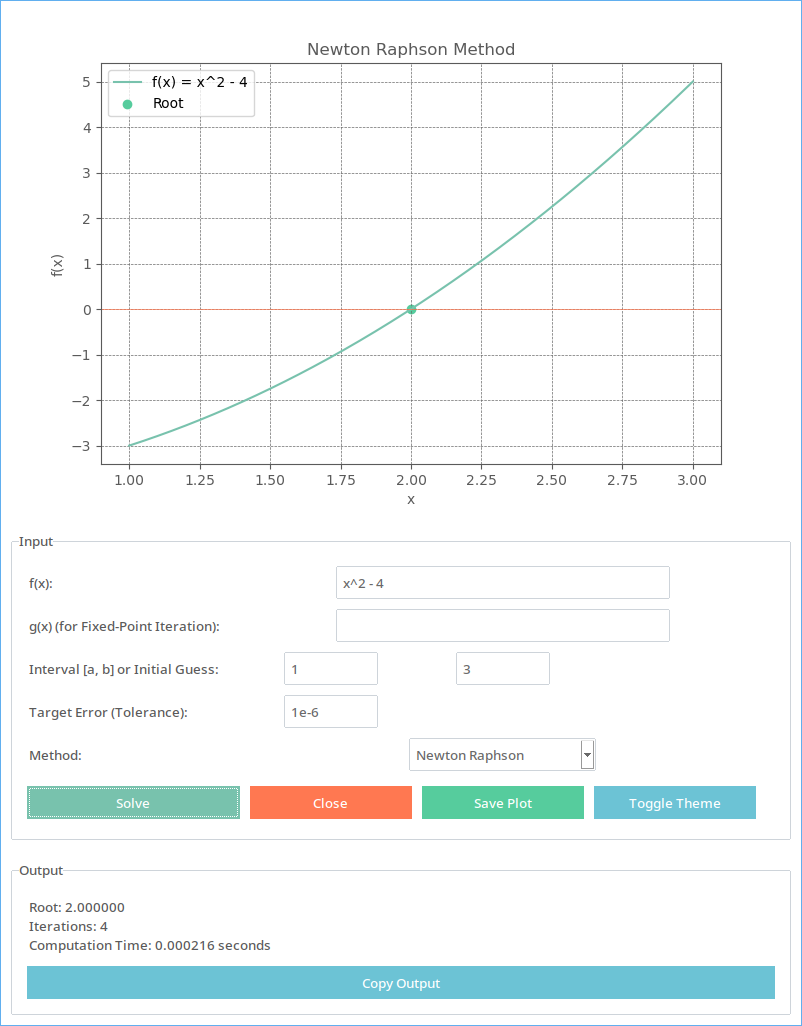
\includegraphics[height=0.5\textwidth]{./fig/demonstracao-app.png}
	\caption{Interface do aplicativo para comparação dos métodos numéricos.}
	\label{fig:demonstracao-app}
\end{figure}
